\documentclass{beamer}
\usepackage{amssymb,amsmath,mathrsfs}
\usepackage{catchfile,etoolbox}

\usepackage{epsfig,psfrag,epstopdf}

\newcommand{\sQ}{\mathcal{Q}}
\newcommand{\sX}{\mathcal{X}}
\newcommand{\nc}{\mathit{nc}}
\DeclareMathOperator*{\argmin}{arg\,min}

\usetheme{Szeged}

\usepackage{graphicx}
\graphicspath{{./figures/}}
\DeclareGraphicsExtensions{.pdf,.eps,.jpg,.png}

\usepackage{es_tutorial}

\usepackage{media9}
\addmediapath{videos}

\title[Energy Shaping]{Orbital Stabilization of Mechanicals Systems}
\subtitle{An Energy Shaping Approach}
\author{R. W. Sinnet}
\institute{Department of Mechanical Engineering\\ Texas A\&M University}
\date{Monday, July 7, 2014}


\begin{document}

\frame{\titlepage}

\begin{frame}
  \frametitle{Overview}
  \tableofcontents[sectionstyle=show,subsectionstyle=hide]
\end{frame}

%\ifdefstring{\PRELIMSECA}{1}{\section{Introduction}
\showtoc

\subsection{Motivation}

\begin{frame}{About Me}
  Ryan W. Sinnet -- Pursuing Ph.D. in Mechanical Engineering
  \begin{itemize}
    \item B.S., Electrical Engineering, Caltech, 2007
    \item M.S., Mechanical Engineering, Texas A\&M, 2011
    \item NSF Graduate Research Fellow, 2010--2013
    \item Valkyrie Humanoid Robot Project, NASA JSC, 2013
  \end{itemize}
\end{frame}

\begin{frame}
  \frametitle{Motivation}
  \begin{block}{Main Idea}
    By understanding energy conservation and energy exchange in mechanical systems with periodic behavior, energy can be shaped using control Lyapunov functions to add robustness to these systems.
  \end{block}
\end{frame}
}{}

\section{Introduction}
\showtoc

\subsection{Motivation}

\begin{frame}{About Me}
  Ryan W. Sinnet -- Pursuing Ph.D. in Mechanical Engineering
  \begin{itemize}
    \item B.S., Electrical Engineering, Caltech, 2007
    \item M.S., Mechanical Engineering, Texas A\&M, 2011
    \item NSF Graduate Research Fellow, 2010--2013
    \item Valkyrie Humanoid Robot Project, NASA JSC, 2013
  \end{itemize}
\end{frame}

\begin{frame}
  \frametitle{Motivation}
  \begin{block}{Main Idea}
    By understanding energy conservation and energy exchange in mechanical systems with periodic behavior, energy can be shaped using control Lyapunov functions to add robustness to these systems.
  \end{block}
\end{frame}

\section{Modeling}
\showtoc

\subsection{Modeling Mechanical Systems}

\begin{frame}
  \frametitle{Generalized Coordinates}
  The smallest set of coordinates that can be used to model a system is called the \blue{generalized coordinates}.
\begin{itemize}
  \item A massive particle requires three coordinates, i.e., $$\sQ \in \R^3.$$
  \item A rigid body requires six coordinates, i.e., $$\sQ \in \R^3 \times \SO = \SE.$$
\end{itemize}
Fewer coordinates can be used on systems with constraints.
\end{frame}


\begin{frame}
  \frametitle{Example: Pendulum on a Cart}

  \begin{figure}
    \centering
    \def\svgwidth{0.8\columnwidth}
    \input{figures/cart_spring.eps_tex}
    \caption{A single coordinate, $x \in \R$, can model a cart with mass $M$ connected to a wall by a spring of stiffness $K$.}
  \end{figure}
\end{frame}


\begin{frame}
  \begin{block}{Newton's Second Law}
    By inspection, the controlled system obeys the dynamics
    \begin{align*}
      M {\ddot x} + K x = F.
    \end{align*}
    This method works on simple systems but does not scale well.
  \end{block}
  
  \begin{block}{Lagrangian Method}
  A more elegant formulation is the method of Lagrange which allows one to obtain a dynamic model by looking at the energy of a system.
  \end{block}
\end{frame}

\begin{frame}
  \frametitle{Lagrangian Systems}
  Mechanical systems are defined by:
  \begin{itemize}
  \item Kinetic energy, $T : T\sQ \to \R^+$,\\
  \item Potential energy, $U : \sQ \to \R$,
  \end{itemize}
  which together comprise the Lagrangian,
  \begin{align*}
    \Lagrangian(q, \dot q) = T(q, \dot q) - U(q).
  \end{align*}
  Dynamical motion in such a system with external forcing $F = B(q) u$ is governed by the Euler--Lagrange equation:
  \begin{align*}
    \frac{d}{dt} \pd{\Lagrangian}{\dq} - \pd{\Lagrangian}{\q} = B(q) u.
  \end{align*}
\end{frame}

\begin{frame}
  \frametitle{Using the Lagrangian Method}
  The cart has kinetic energy $$T(x, {\dot x}) = \frac{1}{2} M {\dot x}^2$$ and potential energy $$U(x) = \frac{1}{2} K x^{2}.$$
The Lagrangian is
\begin{align*}
  \Lagrangian(x, {\dot x}) = \frac{1}{2} M {\dot x}^2 - \frac{1}{2} K x^{2}.
\end{align*}
Applying the Euler--Langrange equation gives
\begin{align*}
  M {\ddot x} + K x = F.
\end{align*}
\end{frame}

\section{Orbital Stabilization}
\showtoc

\subsection{Orbital Stabilization with Control Lyapunov Functions}
\begin{frame}
  \frametitle{Motivation}
  \begin{block}{Main Question}
    Can we use an understanding of energy exchange to improve global stability properties of periodic orbits in mechanical systems?
  \end{block}

  \begin{block}{Observations}
    \begin{itemize}
    \item Numerous control design schemes exist for stabilizing mechanical systems to periodic orbits.
    \item Some controllers produce good behavior locally but lack robustness.
    \item Periodic orbits have associated energy functions with level sets which are invariant under the orbits.
    \end{itemize}
  \end{block}
\end{frame}


\begin{frame}[t]
  \frametitle{Overview}
  \only<1>{
    \begin{block}{Setup}
      Consider the control system 
      \begin{align*}
        \dot x = f(x) + g(x) u(x).
      \end{align*}
      Assume there exists a control law ${\bar u}(x)$ which creates a limit cycle in the closed-loop dynamics,
      \begin{align*}
        {\bar f}(x) = f(\q, \dq) + g(\q) {\bar u}(\q, \dq).
      \end{align*}
      Also assume there exists an energy function $E_{c} : T\ConfigurationSpace \to \R$ which is conserved, i.e., $E_{c}(\q, \dq) \equiv E_{0}$, on the limit cycle.
    \end{block}
  }

  \only<2>{
    \begin{block}{Main Idea}
      Add robustness to a periodic behavior by imposing convergence on an energy function to a level set which is known to be invariant under the system dynamics.
    \end{block}
    
    \begin{block}{Control Objective}
      Choose control input $\mu(\q, \dq)$ such that $\| \mu(\q, \dq) - {\bar u}(\q, \dq) \|$ is minimized and $E_{c}(\q(t), \dq(t)) \to E_0$ as $t \to \infty$.
    \end{block}

    \begin{block}{Exponential Convergence}
      To achieve exponential stabilization, $E_{c}(x(t))$ should satifisy
      \begin{align*}
        E_{c}(\q(t), \dq(t)) \leq E_{c}(\q(t_{0}), \dq(t_{0})) e^{-\beta t} \mbox{ for } t \geq t_{0}, \beta > 0.
      \end{align*}
    \end{block}
  }
\end{frame}

\begin{frame}
  \frametitle{Control Lyapunov Functions}
  A \blue{control Lyapunov function} $V : X \to \R$ which satisfies
  \begin{align*}
    &c_{1} \| x \|^2 \leq V(x) \leq c_{2} \|x\|^2,\\
    &\inf_{u \in U} L_f V(x) + L_g V(x) \, u + c_{3} V(x) \leq 0
  \end{align*}
  for $c_{1}, c_{2}, c_{3} > 0$ exhibits exponential convergence.
\end{frame}

\begin{frame}
  \frametitle{Energy Shaping}
  Consider a conserved energy function $E_{c}(x)$. For an exponentially stablilzing CLF, we seek $\mu(x)$ such that
  \begin{align*}
    L_f V(x) + L_g V(x) \, \mu(x) + \epsilon V(x) &\leq 0.
  \end{align*}
  Choosing $V(x) = \eta^2$ with $\eta(x) = E_{c}(x) - E_{0}$, we obtain
  \begin{align*}
    2 \eta(x) \left(L_f \eta(x) + L_g \eta(x) \, \mu(x) \right) + \epsilon \eta^2(x) \leq 0.
  \end{align*}
  We can relax this condition by augmenting the optimization space with $\delta \in \R$ and requiring
  \begin{align*}
    2 \eta(x) \left(L_f \eta(x) + L_g \eta(x) \, \mu(x) \right) + \epsilon \eta^2(x) \leq \delta(x).
  \end{align*}
\end{frame}

\begin{frame}[t]
  \frametitle{Quadratic Program Formulation}
  The linear form of the CLF condition suggests
  \begin{align}
    \nonumber
    (\delta^*(x), \mu(x)) = \argmin_{v = (\delta, u)}  \, & v^T \! H \, v + h^T(x) v\\
    \label{clf} \tag{clf}
    \mbox{s.t. } & \Aclf(x) \, v \leq \bclf(x)%\\
    %\label{lim} \tag{lim}
    %& \Alim v \leq \blim
  \end{align}
  where \eqref{clf} imposes the control Lyapunv function. To encode the dynamics of the system under control input ${\bar u}(x)$, select
  \begin{align*}
    H = \left(\begin{array}{c c}\nu & 0\\ 0 & I\end{array}\right), & \quad
      h(x) = \left(\begin{array}{c} 0\\ -2 \, \bar u(x) \end{array}\right),\\
      \Aclf = \left(\begin{array}{c c}
        -1 & 2 \eta(x) \, L_{g} \eta(x)
      \end{array}\right), & \quad
      \bclf = -\epsilon \eta^{2}(x) - 2\eta(x) \, L_{f} \eta(x).
  \end{align*}
  with positive weighting coefficient $\nu \in \R$.
\end{frame}

\begin{frame}[t]
  \frametitle{Example: Cart with Spring}
  \only<1>{
   \begin{figure}
      \centering
      \def\svgwidth{0.8\columnwidth}
      \input{figures/cart_spring.eps_tex}
      \caption{A single coordinate, $x \in \R$, can model a cart with mass $M$ connected to a wall by a spring of stiffness $K$.}
    \end{figure}
  }

  \only<2>{
    Consider the Lypaunov candidate function
    \begin{align*}
      V(x, \dot x) = (E(x, {\dot x}) - E_{0})^{2}
    \end{align*}
    where $$E(x, {\dot x}) = \frac{1}{2} M {\dot x}^2 + \frac{1}{2} K x^2.$$
    Differentiation gives
    \begin{align*}
      {\dot V}(x, {\dot x}) = 2\left(E(x, {\dot x}) - E_{0}\right) {\dot E}(x, {\dot x})
    \end{align*}
    Under control input $u$,
    \begin{align*}
      {\dot E}(x, {\dot x}) =  L_{f}(x, {\dot x}) + L_{g} E(x, {\dot x}) u.
    \end{align*}
  }

  \only<3>{
    The Lyapunov function $V(x)$ in
    \begin{align*}
      \epsilon V(x, {\dot x}) + 2\left(E(x, {\dot x}) - E_{0}\right) \left(L_{f} E(x, {\dot x}) + L_{g} E(x, {\dot x}) u \right) \leq 0
    \end{align*}
    includes $u$ and is called a control Lyapunov function. The Lie derivatives are
    \begin{align*}
      L_{f} E(x, {\dot x}) &= \pd{E(x, {\dot x})}{x} {\dot x} + \pd{E(x, {\dot x})}{{\dot x}} \left(-\frac{K}{M} x\right)\\
      &= K x \dot x - K x {\dot x} = 0,\\
      L_{g} E(x, {\dot x}) &= \pd{E(x, {\dot x})}{{\dot x}} \frac{1}{M}\\
      &= \frac{K}{M} x.
    \end{align*}
  }

  \only<4>{
    Energy shaping is achieved by applying the following control law:
    \begin{align*}
      \mu(x, {\dot x}) = \argmin_{u \in \R} \, & u^T u\\
      \mbox{s.t. } & \Aclf(x, {\dot x}) \, u \leq \bclf(x, {\dot x})%\\
    \end{align*}
    where
    \begin{align*}
      \Aclf(x, {\dot x}) &= 2(E(x, {\dot x}) - E_{0}) \frac{K}{M} x,\\
      \bclf(x, {\dot x}) &= -\epsilon(E(x, {\dot x})- E_{0})^2.
    \end{align*} 
  }

  \only<5>{
    \begin{figure}
      \centering
      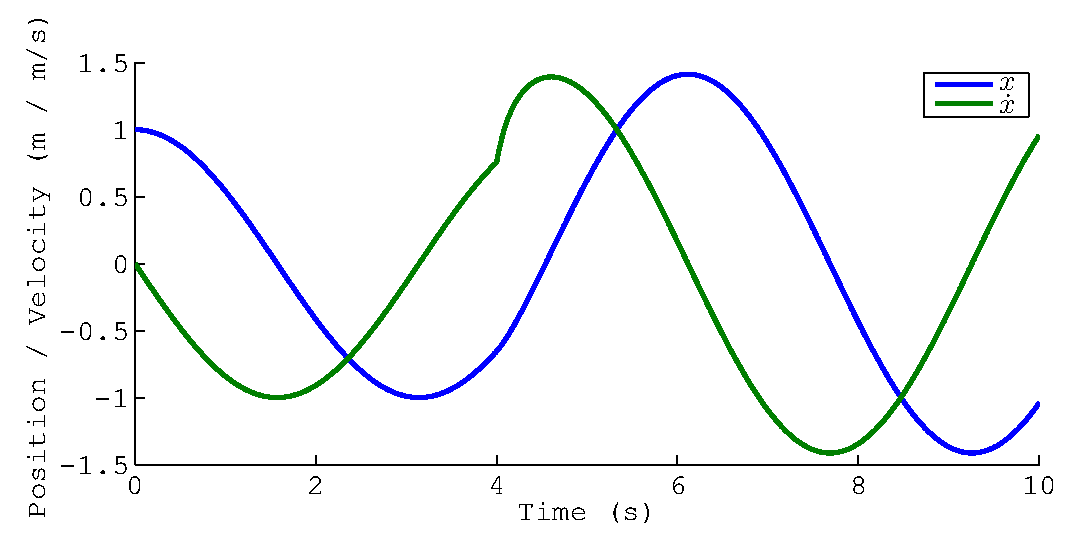
\includegraphics[width=0.8\columnwidth]{cart_spring_es}
      \caption{Energy shaping can shift the cart between energy levels. The difference is evidence in the amplitude of the solution.}
    \end{figure}
  }

  \only<6>{
    \begin{figure}
      \centering
      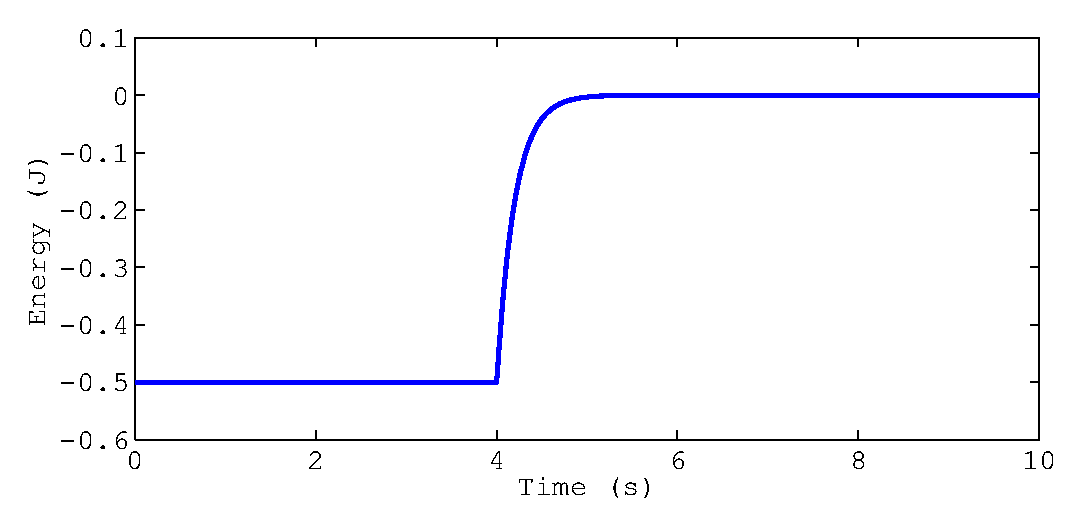
\includegraphics[width=0.8\columnwidth]{cart_spring_es_energy}
      \caption{The transition between energy levels demonstrates exponential convergence.}
    \end{figure}
  }

  \only<7>{
    \begin{figure}
      \centering
      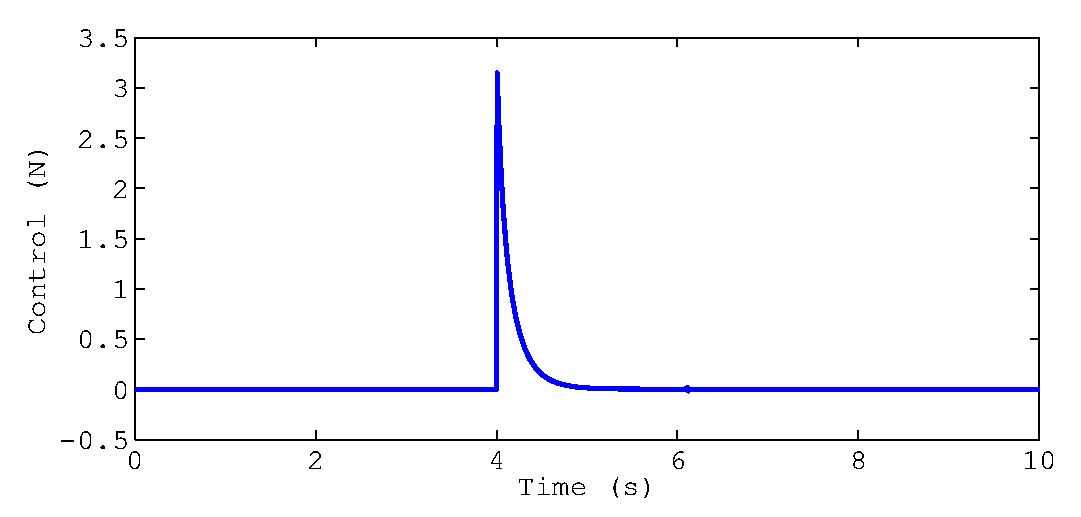
\includegraphics[width=0.8\columnwidth]{cart_spring_es_control}
      \caption{The controller applies feedback to converge to the desired energy level. Discontinuous control can be avoided with conditions on the optimization problem.}
    \end{figure}
  }
\end{frame}


\section{Hybrid Systems}
\showtoc

\subsection{Modeling}

\begin{frame}
  \frametitle{Modeling Hybrid Systems}
  \begin{columns}
    \begin{column}{.63\textwidth}
      \begin{definition}
        A \alert{hybrid control system} is a tuple \vspace{-.3cm}
        $$\HCS = \hcsystem, \vspace{-.4cm}$$
        where
        \begin{itemize}
        \item
          $\Domain \subset \mathcal{X}$ is the \blue{domain of admissibility} with state space $\mathcal{X}$,
        \item
          $\ControlSet$ is a set of \blue{admissible controls},
        \item
          $\Guard$ is a \blue{guard} or \blue{switching surface},
        \item
          $\ResetMap$ is a smooth \blue{reset map},
        \item
          $(f, g)$ is a \blue{control system} on $\Domain$: \vspace{-3mm}
          \begin{align*}
            \dot{x} = f(x) + g(x) \, u.
          \end{align*}
        \end{itemize}
      \end{definition}
    \end{column}
    \begin{column}{.4\textwidth}
      \begin{figure}
        \centering
        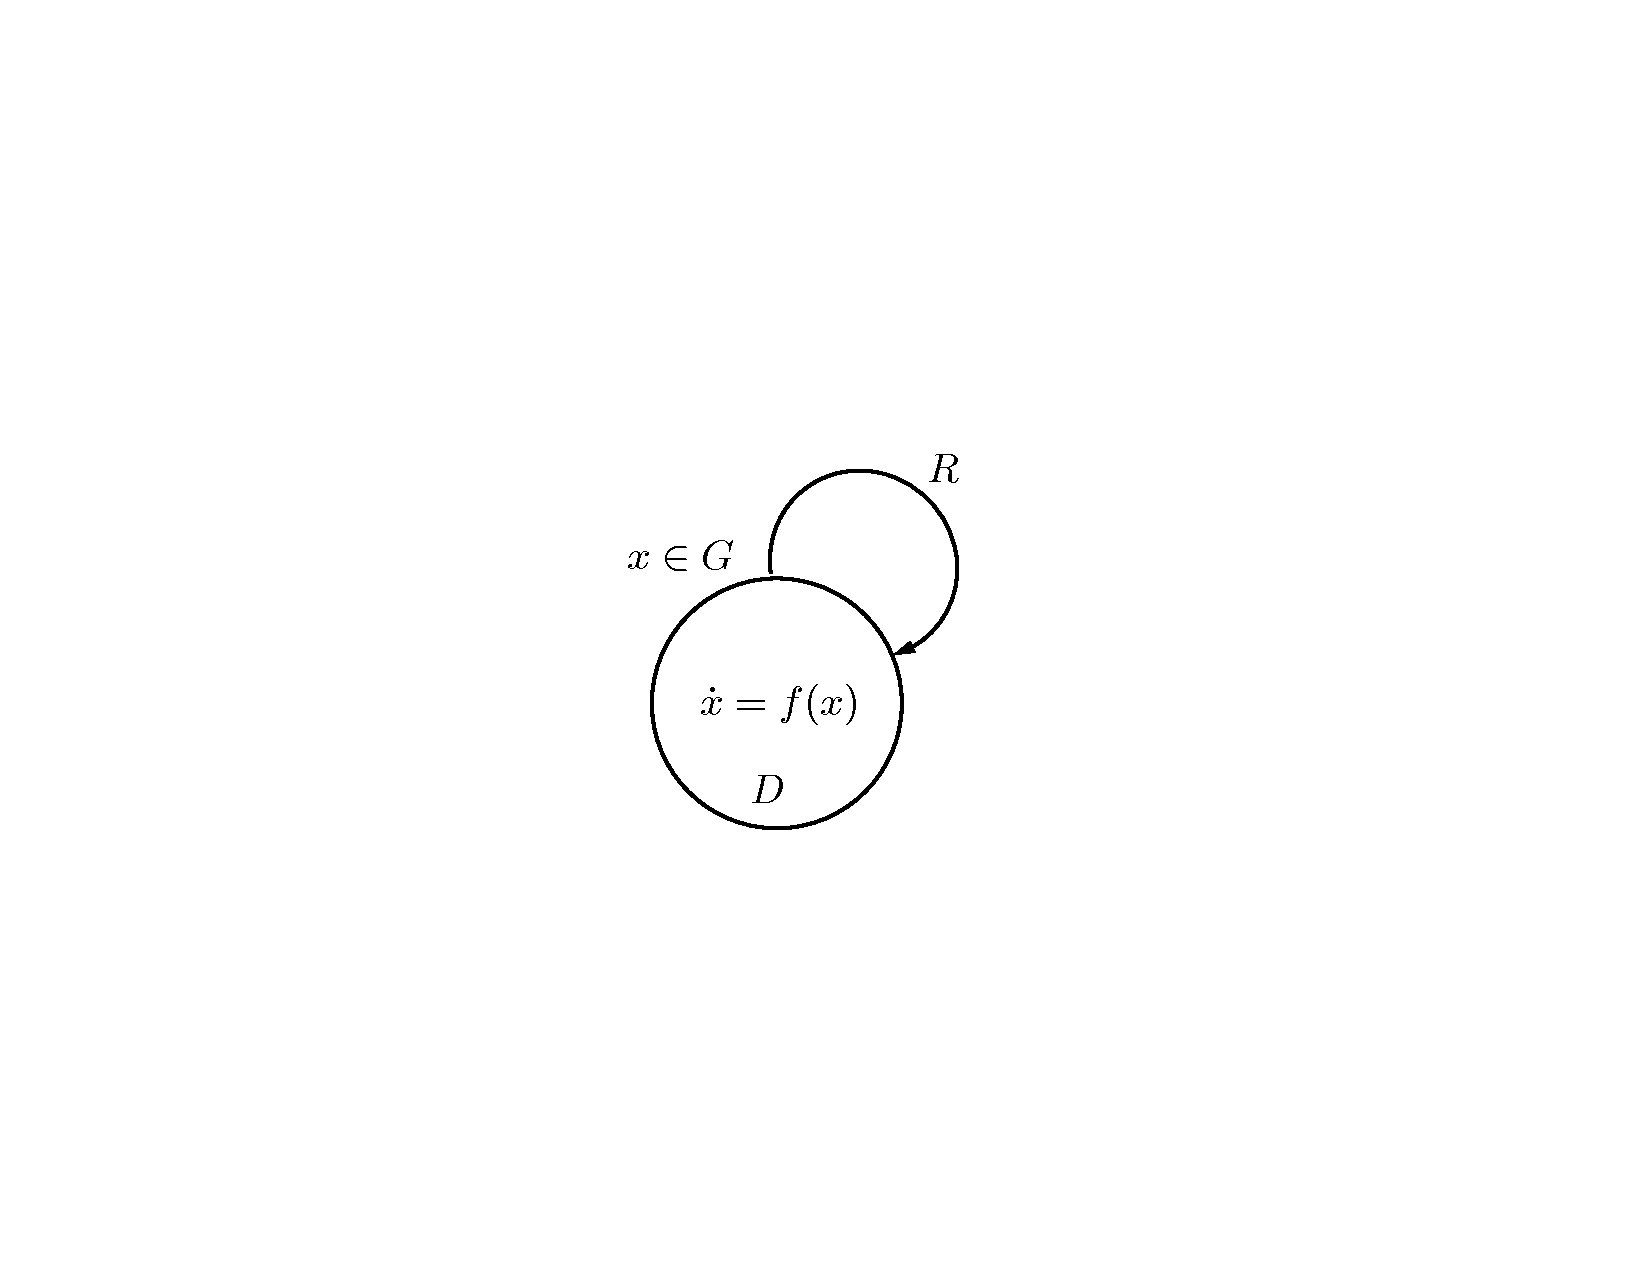
\includegraphics[width=.9\textwidth]{hsystem}\\
      \end{figure}
      A \alert{simple hybrid system}:\vspace{-.3cm}
      $$\HS = \hsystem$$
    \end{column}
  \end{columns}
\end{frame}

\begin{frame}
  \frametitle{Swing Phase Dynamics}
  \begin{columns}
    \begin{column}{.55\textwidth}
      For Lagrangian $\Lagrangian$ with coordinates
      \begin{align*}
        x = (\q^{T}, \dq^{T})^{T} \in T\ConfigurationSpace,
      \end{align*}
      the dynamic model has the form
      \begin{align*}
        \D(\q) \, \ddq + \C(\q, \dq) \, \dq + \G(\q) = B(\q) \, u,
      \end{align*}
      or $\dot x = f(q, \dot q) + g(q) \, u,$ with
      \begin{align*}
        f(\q, \dq) &= \left(\!\!\begin{array}{c}
        \dq\\
        \D^{-1}(\q) (-\C(\q, \dq) \, \dq - \G(\q))
        \end{array}\!\!\right),\\
        g(\q) &= \left(\!\!\begin{array}{c}
        \mathbf{0}_{m \times m}\\
        \D^{-1}(\q) B(\q)
        \end{array}\!\!\right).
      \end{align*}
    \end{column}\!\!
    \begin{column}{.45\textwidth}
      \begin{figure}
        \centering
        \vspace{-10mm}
        \caption{Physical configuration}
        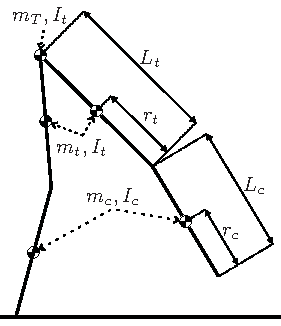
\includegraphics[width = 1.0\columnwidth]{robot_config}
      \end{figure}
    \end{column}
  \end{columns}
\end{frame}

\begin{frame}
  \frametitle{Impact Dynamics}
  Introduce extended coordinates $\qe = (X, \q^{T})^{T} \in \mathrm{SE}(3) \times \ConfigurationSpace$ which contains the kinematics of a reference point on the robot. Angular momentum balance based on H{\"u}rm{\"u}zl{\"u} and Marghitu:
  \begin{massump}
    \begin{itemize}
    \item Rigid-body plastic impacts
    \item Enough friction to prevent slipping
    \item Motors do not produce impulses
    \item No instantaneous change in configuration, i.e., $\qe^{-} = \qe^{+}$
    \end{itemize}
  \end{massump}
  Under these assumptions, the discrete dynamics satisfies
  \begin{align*}
    \left[\begin{array}{c c}
        \D_{e}(\qe) & -\Jacobian^{T}(\qe)\\
        \Jacobian(\qe) & \mathbf{0}_{3 \times 3}
      \end{array}\right]
    \left[\begin{array}{c}
        \dq^{+}\\
        \delta F(\qe, \dqe)
      \end{array}\right]
    = \left[\begin{array}{c c}
        \D_{e}(\qe) \, \dqe^{-}\\
        \mathbf{0}_{3}
      \end{array}\right].
  \end{align*}
\end{frame}

\subsection{Solutions to Hybrid Systems}
\begin{frame}[t]
  \frametitle{Hybrid Flows}
  A \alert{hybrid flow} of $\HS$ is a tuple
  \begin{align*}
    \chi^{\HS} = \left( \Delta, \mathscr{I}, \mathscr{C} \right),
  \end{align*}
  \vspace{-2em}
  \begin{itemize}
  \item $\Delta = \{0, 1, 2, \ldots\} \subseteq \Nat$ is a finite or infinite \blue{indexing set},
  \item $\mathscr{I} = \{I_{i} \}_{i \in \Delta}$ is a \blue{hybrid interval} where $I_{i} = [\tau_{i}, \tau_{i + 1}]$,
  \item $\mathscr{C} = \{c_{i} \}_{i \in \Delta}$ is a \blue{collection of solutions} of $f$, i.e., ${\dot c}_{i}(t) = f(c_{i}(t))$ $\forall i \in \Delta$.
  \end{itemize}

  \only<1>{
    \vspace{-1em}
    \begin{figure}
      \centering
      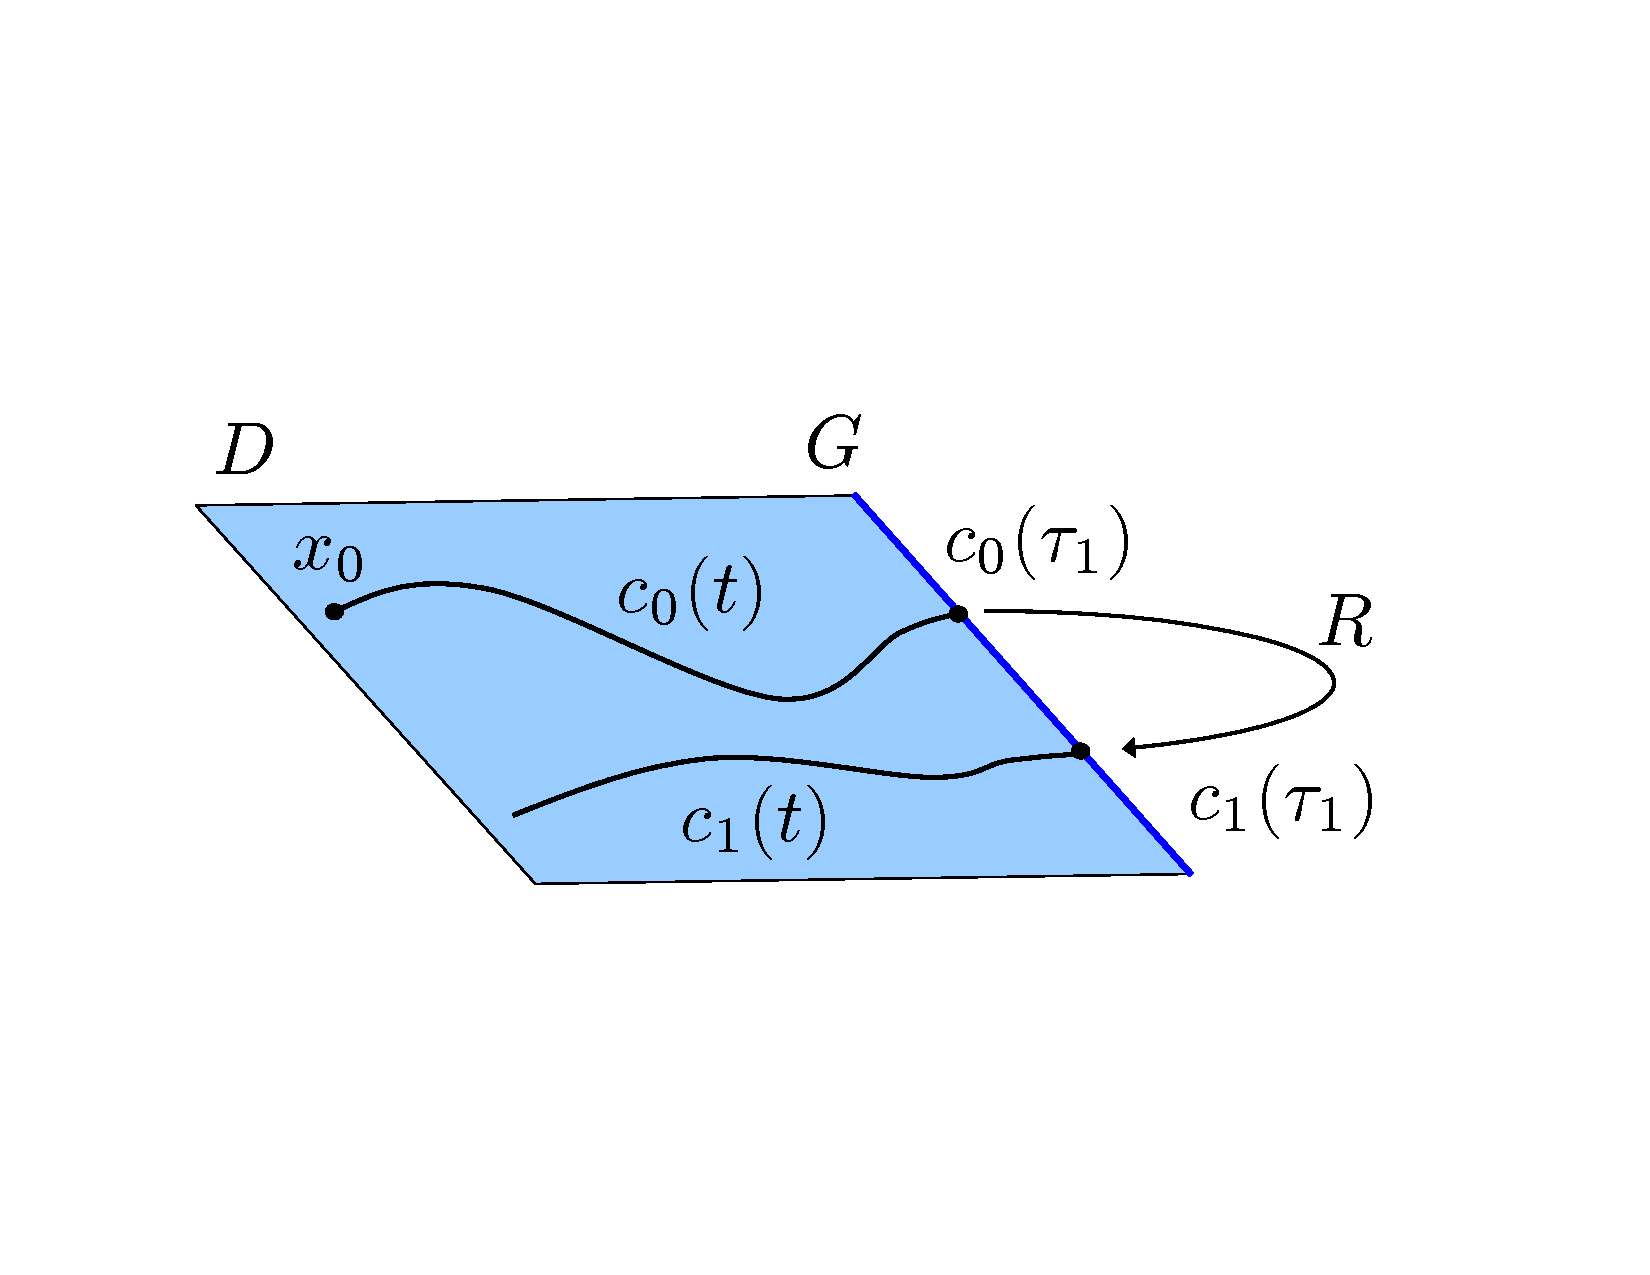
\includegraphics[width=0.5\columnwidth]{hybridflow}
    \end{figure}
    \vspace{-1em}
  }

  \only<2>{
    In addition, for every $i, i + 1 \in \Delta$, it is required that
    \begin{enumerate}
    \item $c_{i}(\tau_{i+1}) \in G$ and
    \item $\Delta(c_{i}(\tau_{i+1})) = c_{i+1}(\tau_{i+1})$
    \end{enumerate}
  }
\end{frame}


\begin{frame}
  \frametitle{Periodic Orbits}
  \begin{figure}    
    \centering
    \def\svgwidth{.45\columnwidth}
    \input{figures/hybrid_periodic_orbit.eps_latex}
    \caption{A hybrid periodic orbit. Stability is ascertained using the method of Poincar\'e.}
  \end{figure}
\end{frame}

\begin{frame}
  \frametitle{Conservative Systems}
  For a conservative system, total energy is conserved; i.e.:
  \begin{align*}
    E_{c} &= T(q, \dot q) + U(q)\\
    &= E(q(0), \dot q(0)) = E_{0}
  \end{align*}
  Dynamical motion for such a system relies on the interplay between kinetic and potential energy, which is expressed in the Euler-Lagrange equation,
  \begin{align*}
    \frac{d}{dt} \pd{\Lagrangian}{\dq} - \pd{\Lagrangian}{\q} = 0.
  \end{align*}
\end{frame}


\begin{frame}
  \frametitle{The Simplest Example: Passive Compass-Gait Biped}
  \only<1>{
    \begin{columns}
      \column{1.5in}
      Dynamic Model:
      \begin{align*}
        M(q) \ddot q + H(q, \dot q) = 0
      \end{align*}
      Control Law:
      \begin{align*}
        u = 0.
      \end{align*}
      \column{1.5in}
      \begin{figure}%width=1.0\columnwidth,
        
        \centering
        \def\svgwidth{1.0\columnwidth}
        \input{figures/cg2d-slope-model.eps_latex}
        \vspace{-2em}
        \caption{Compass-gait biped falling down a slope.}
      \end{figure}
    \end{columns}
  }

  \only<2>{
    \begin{figure}
      \includemedia[
        %width=1.0\columnwidth,
        %height=0.5625\columnwidth,
        width=1.0\columnwidth,
        height=0.5\columnwidth,
        addresource=cg2d_slope.mp4,
        activate=pageopen,
        flashvars={source=cg2d_slope.mp4&loop=true&autoPlay=true}
      ]{}{VPlayer9.swf}
      \caption{Stable passive gaits can be found for a range of slopes.}
    \end{figure}    
  }

  \only<3>{
    \begin{figure}
      \centering
      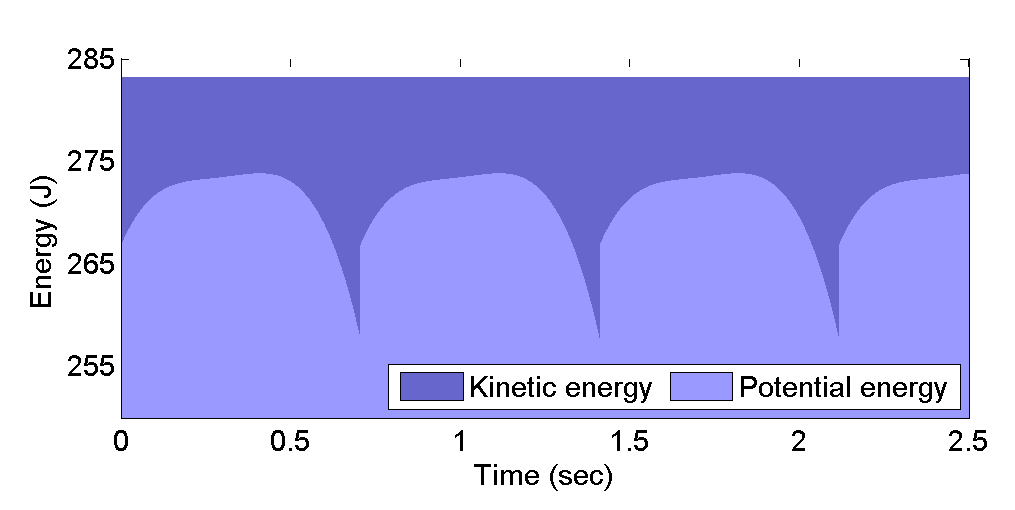
\includegraphics[width=1.0\columnwidth]{energy_cg2d_slope_model}
      \caption{Energy is exchanged between kinetic and potential in form.}
    \end{figure}    
  }
\end{frame}


\begin{frame}
  \frametitle{Nonconservative Systems}
  For a nonconservative system, energy flows out of the system at a rate of $F_{\nc} \cdot dq$. Thus, the following quantity is conserved:
  \begin{align*}
    E_{c} &= T(q, \dot q) + U(q) - \int_{t_{0}}^{t} \! F_{\nc} \cdot \frac{dq}{d\tau} \ d\tau\\
    &= E(q(0), \dot q(0)) = E_{0}
  \end{align*}
  This equation expresses the interplay between kinetic and potential energy and the flow of energy into and out of the system.
\end{frame}


\begin{frame}
  \frametitle{Example: Active Compass-Gait Biped}
  \only<1>{
    \begin{columns}
      \column{1.5in}
      Dynamic Model:
      \begin{align*}
        M(q) \ddot q + H(q, \dot q) = B(q) u.
      \end{align*}
      Controlled Symmetries:
      \begin{align*}
        u &= G(q) - G(\Psi_{\gamma}(q))
      \end{align*}
      where $\Psi : \S \times \R \to \sQ$ rotates the frame of gravity by $\gamma$.

      \column{1.5in}
      \begin{figure}
        \centering
        \def\svgwidth{1.0\columnwidth}
        \input{figures/cg2d-2link-model.eps_latex}
        \vspace{-2em}
        \caption{Compass-gait biped with Controlled Symmetries.}
      \end{figure}
    \end{columns}
  }
  \only<2>{
    \begin{figure}
      \includemedia[
        %width=1.0\columnwidth,
        %height=0.5625\columnwidth,
        width=1.0\columnwidth,
        height=0.5\columnwidth,
        addresource=cg2d_2link_simulation.mp4,
        activate=pageopen,
        flashvars={source=cg2d_2link_simulation.mp4&loop=true&autoPlay=true}
      ]{}{VPlayer9.swf}
      \caption{Passive downhill gaits can be translated to flat ground with Controlled Symmetries.}
    \end{figure}    
  }
  \only<3>{
    \begin{figure}
      \centering
      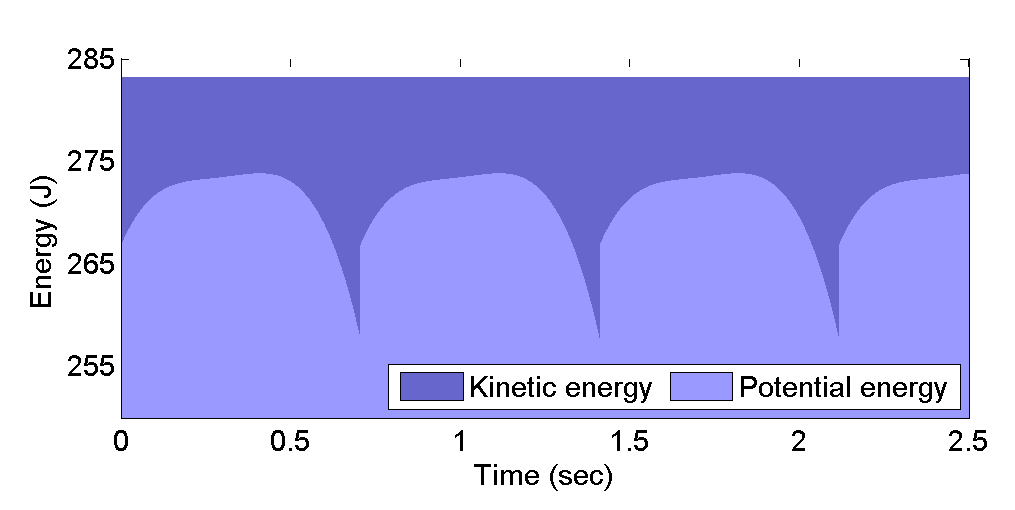
\includegraphics[width=1.0\columnwidth]{energy_cg2d_slope_model}
      \caption{Energy of the shaped system is conserved.}
    \end{figure}    
  }
\end{frame}

\begin{frame}
  \frametitle{Example: 3-Link Biped}
  \only<1>{
    \begin{columns}
      \column{1.5in}
      Dynamic Model:
      \begin{align*}
        M(q) \ddot q + H(q, \dot q) = B(q) u
      \end{align*}
      Control Law:
      \begin{align*}
        u &= G(q) - G(\Psi(q))\\
        u_3 &=-k_{d} (\dot \vartheta_{T}^{a})\\
        &\hspace{1.8em} -k_{p} (\vartheta_{T}^{a} - \vartheta_{T}^{d})
      \end{align*}
      \column{1.5in}
      \begin{figure}
        \centering
        \def\svgwidth{1.0\columnwidth}
        \input{figures/cg2d-3link-model.eps_latex}
        \vspace{-2em}
        \caption{3-link biped configuration.}
      \end{figure}
    \end{columns}
  }

  \only<2>{
    \begin{figure}
      \centering
      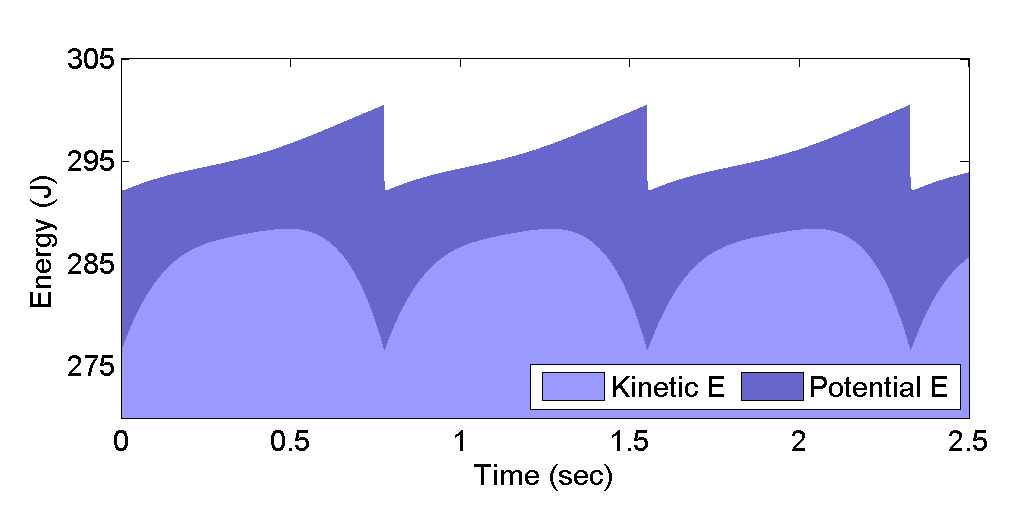
\includegraphics[width=1.0\columnwidth]{energy_cg2d_3link}
      \caption{Energy is not conserved as the controller injects energy.}
    \end{figure}
  }

  \only<3>{
    \begin{figure}
      \includemedia[
        width=1.0\columnwidth,
        height=0.5\columnwidth,
        addresource=cg2d_3link_simulation.mp4,
        activate=pageopen,
        flashvars={source=cg2d_3link_simulation.mp4&loop=true&autoPlay=true}
      ]{}{VPlayer9.swf}
      \caption{Stable passive gaits can be found for a range of slopes.}
    \end{figure}
  }
\end{frame}

\section{Conclusion}
\showtoc

\subsection{Concluding Remarks}

\begin{frame}
  \frametitle{Summary}
  \begin{block}{Energy Shaping}
    Provides an intuitive approach for adding robustness to mechanical systems through control:
    \begin{itemize}
      \item Based on Lyapunov's method
      \item Allows one to impose dynamic constraints
      \item Quick to solve due to convex nature of problem
      \item Can be applied to a wide range of systems
    \end{itemize}
  \end{block}

  \begin{block}{Open Questions}
    \begin{itemize}
    \item Can energy shaping be used to stabilize unstable systems?
    \item Is this method robust for practical implementations?
    \end{itemize}
  \end{block}
\end{frame}

\begin{frame}
  \frametitle{Questions?}

  Thank you for listening.
\end{frame}


\end{document}
